\documentclass{article}

% Language setting
% Replace `english' with e.g. `spanish' to change the document language
\usepackage[english]{babel}

\usepackage[letterpaper,top=2cm,bottom=5cm,left=3cm,right=3cm,marginparwidth=1.75cm]{geometry}

% Useful packages
\usepackage{amsmath}
\usepackage{graphicx}
\usepackage[colorlinks=true, allcolors=blue]{hyperref}
\usepackage{amssymb} 
\usepackage{fancyhdr}
\usepackage{lipsum} % Para generar texto de ejemplo
\usepackage{multicol}
\usepackage{array}
\usepackage{enumitem}
\usepackage{float}
\pagestyle{fancy} 



\fancyhf{} % Limpiar encabezado y pie de página por defecto
\setlength{\headheight}{85pt} % Ajuste del tamaño del encabezado

% Definición del encabezado
\fancyhead[C]{%
    \begin{minipage}[c]{1.5cm}
        
\includegraphics[width=1.5cm]{imagenes/uta.png}
    \end{minipage}%
    \hfill  % <--- SIN EL SIGNO % (descomentado)
    \begin{minipage}[c]{10cm} 
        \centering
        \small \textbf{UNIVERSIDAD TÉCNICA DE AMBATO}\\[0.1cm]
        \scriptsize \textit{FACULTAD DE INGENIERÍA EN SISTEMAS, ELECTRÓNICA E INDUSTRIAL}\\[0.1cm]
        \scriptsize \textbf{CARRERA SOFTWARE - BASE DE DATOS}\\[0.1cm]
        \scriptsize \textbf{CICLO ACADÉMICO: ENERO 2026 - JULIO 2026}\vspace{0.3cm}
    \end{minipage}%
    \hfill  % <--- SIN EL SIGNO % (descomentado)
    \begin{minipage}[c]{1.5cm}
        \centering
        
\includegraphics[width=1.5cm]{imagenes/fisei.png}
    \end{minipage}%
}


\begin{document}
\begin{center}
    {\large \textbf{INFORME DE GUÍA PRÁCTICA}} \\    
\end{center}

\section{Portada}
\begin{flushleft}
\begin{tabular}{>{\bfseries}p{6.2cm} p{8.5cm}}
Tema: & Proyecto del Primer Parcial \\
Unidad de Organización Curricular: & PROFESIONAL \\
Nivel y Paralelo: & 4to Semestre ``B'' \\
Alumno participante: & Guatemal Avilez Bryan Stalin \\
& Bejarano Masabanda Carlos Fabian \\
& Molina Nuñez Karen Valeria \\
& Espín Caiza Camila Gisselle \\

Asignatura: & Base de Datos \\
Docente: & Ing. Jose Ruben Caiza Caizabuano Mg. \\
Modalidad: & Presencial \\
\end{tabular}
\end{flushleft}


\section{Informe de guía práctica}
\subsection{Objetivos}
\subsubsection{General}
Diseñar e implementar un sistema web de gestión de inventario tecnológico para la FISEI.
\subsubsection{Específicos}
\begin{itemize}
    \item Levantar requerimientos
    \item Definir entidades, relaciones y reglas
    \item Construir modelo ER
    \item Transformar a modelo relacional
    \item Aplicar normalización
    \item Implementar en Oracle
\end{itemize}
\subsection{Modalidad}
Presencial

\subsection{Tiempo de duración}

Presenciales: 0\\
No presenciales: 4




\subsection{Listado de equipos, materiales y recursos}
\textbf{Listado de equipos y materiales generales empleados en la guía práctica:}
\begin{itemize}
    \item Oracle Database
\end{itemize}

\textbf{TAC (Tecnologías para el Aprendizaje y Conocimiento) empleados en la guía práctica:}
\begin{itemize}
    \item[$\square$] Plataformas educativas
    \item[$\square$] Simuladores y laboratorios virtuales
    \item[$\square$] Aplicaciones educativas
    \item[$\square$] Recursos audiovisuales
    \item[$\square$] Gamificación
    \item[$\square$] Inteligencia Artificial
    \item Otros (Especifique): \underline{\hspace{5cm}}
\end{itemize}




\section{Introducción}

La Facultad de Ingeniería en Sistemas, Electrónica e Industrial administra equipos tecnológicos distribuidos en laboratorios, aulas y oficinas. El control manual de estos bienes dificulta el seguimiento de su ubicación, la trazabilidad de los mantenimientos, el control de préstamos y la generación de reportes oportunos. Por ello se propone un sistema integral que permita registrar, consultar, prestar, mantener y auditar los activos tecnológicos mediante una solución web apoyada en una base de datos relacional implementada en Oracle.

El presente proyecto ha sido diseñado como una guía académica integral. Su propósito no es únicamente crear tablas, sino llevar al estudiante a comprender la secuencia completa del diseño de datos: identificación del problema, levantamiento de requerimientos, formulación de reglas de negocio, diseño conceptual, transformación al modelo lógico relacional, normalización, implementación física en Oracle y construcción de una interfaz amigable para el usuario final.

\section{Planteamiento del problema}

En la gestión cotidiana del inventario tecnológico surgen dificultades recurrentes: pérdida de información, inconsistencias en el registro de bienes, desconocimiento del estado real de los artículos, demoras para ubicar equipos disponibles, ausencia de historial de mantenimientos y carencia de alertas sobre devoluciones próximas.

Tales problemas afectan la eficiencia operativa y la toma de decisiones en la institución.

La solución propuesta consiste en desarrollar un sistema web con una arquitectura modular y una base de datos Oracle que centralice toda la información del inventario.
\section{Alcance funcional del sistema}

El sistema permitirá gestionar:

\begin{itemize}
    \item Inventario de equipos
    \item Ubicaciones
    \item Préstamos y devoluciones
    \item Mantenimientos
    \item Notificaciones
    \item Auditoría
\end{itemize}

\section{Situación (resumen)}

En la gestión cotidiana del inventario tecnológico surgen dificultades recurrentes: pérdida de información, inconsistencias en el registro de bienes, desconocimiento del estado real de los artículos, demoras para ubicar equipos disponibles, ausencia de historial de mantenimientos y carencia de alertas sobre devoluciones próximas. Tales problemas afectan la eficiencia operativa y la toma de decisiones en la institución. La solución propuesta consiste en desarrollar un sistema web con una arquitectura modular y una base de datos Oracle que centralice toda la información del inventario. El sistema debe ser capaz de soportar el registro de equipos, el control de ubicaciones, la gestión de responsables, préstamos, devoluciones, notificaciones, mantenimientos y trazabilidad de las acciones ejecutadas por los usuarios.

\section{Entidades importantes}

\begin{itemize}[leftmargin=1.5cm]
    \item Usuario
    \item Rol
    \item Artículo
    \item Categoría
    \item Ubicación
    \item Departamento
    \item Préstamo
    \item Detalle\_Préstamo
    \item Mantenimiento
    \item Movimiento
    \item Notificación
    \item Auditoría
\end{itemize}

\section{Atributos principales}

\subsection{Usuario}
\begin{itemize}
    \item id\_usuario (PK)
    \item nombre
    \item correo
    \item contraseña
    \item id\_rol (FK)
\end{itemize}

\subsection{Rol}
\begin{itemize}
    \item id\_rol (PK)
    \item nombre\_rol
\end{itemize}

\subsection{Artículo}
\begin{itemize}
    \item id\_articulo (PK)
    \item nombre
    \item estado
    \item codigo
    \item id\_categoria (FK)
    \item id\_ubicacion (FK)
    \item id\_responsable (FK opcional)
\end{itemize}

\subsection{Categoría}
\begin{itemize}
    \item id\_categoria (PK)
    \item nombre
\end{itemize}

\subsection{Ubicación}
\begin{itemize}
    \item id\_ubicacion (PK)
    \item nombre
    \item id\_departamento (FK)
\end{itemize}

\subsection{Departamento}
\begin{itemize}
    \item id\_departamento (PK)
    \item nombre
\end{itemize}

\subsection{Préstamo}
\begin{itemize}
    \item id\_prestamo (PK)
    \item fecha\_prestamo
    \item fecha\_devolucion
    \item id\_usuario (FK)
\end{itemize}

\subsection{Detalle\_Préstamo}
\begin{itemize}
    \item id\_detalle (PK)
    \item id\_prestamo (FK)
    \item id\_articulo (FK)
\end{itemize}

\subsection{Mantenimiento}
\begin{itemize}
    \item id\_mantenimiento (PK)
    \item tipo
    \item fecha
    \item id\_articulo (FK)
\end{itemize}

\subsection{Movimiento}
\begin{itemize}
    \item id\_movimiento (PK)
    \item fecha
    \item tipo
    \item id\_articulo (FK)
\end{itemize}

\subsection{Notificación}
\begin{itemize}
    \item id\_notificacion (PK)
    \item mensaje
    \item estado
    \item id\_prestamo (FK)
\end{itemize}

\subsection{Auditoría}
\begin{itemize}
    \item id\_auditoria (PK)
    \item accion
    \item fecha
    \item id\_usuario (FK)
\end{itemize}

\section{Relaciones}

\begin{itemize}
    \item Usuario $\rightarrow$ pertenece a $\rightarrow$ Rol
    \item Artículo $\rightarrow$ pertenece a $\rightarrow$ Categoría
    \item Artículo $\rightarrow$ está en $\rightarrow$ Ubicación
    \item Ubicación $\rightarrow$ pertenece a $\rightarrow$ Departamento
    \item Préstamo $\rightarrow$ tiene $\rightarrow$ Detalle\_Préstamo
    \item Artículo $\rightarrow$ participa en $\rightarrow$ Detalle\_Préstamo
    \item Artículo $\rightarrow$ tiene $\rightarrow$ Mantenimiento
    \item Artículo $\rightarrow$ tiene $\rightarrow$ Movimiento
    \item Préstamo $\rightarrow$ genera $\rightarrow$ Notificación
    \item Usuario $\rightarrow$ genera $\rightarrow$ Auditoría
\end{itemize}

\section{Cardinalidades}

\begin{itemize}
    \item Rol (1) ------ (N) Usuario
    \item Departamento (1) ------ (N) Ubicación
    \item Categoría (1) ------ (N) Artículo
    \item Ubicación (1) ------ (N) Artículo
    \item Préstamo (1) ------ (N) Detalle\_Préstamo
    \item Artículo (1) ------ (N) Detalle\_Préstamo
    \item Artículo (1) ------ (N) Mantenimiento
    \item Artículo (1) ------ (N) Movimiento
    \item Préstamo (1) ------ (N) Notificación
    \item Usuario (1) ------ (N) Auditoría
\end{itemize}

\section{Participación}

\begin{itemize}
    \item Usuario $\rightarrow$ participación total en Rol
    \item Artículo $\rightarrow$ participación total en Categoría y Ubicación
    \item Préstamo $\rightarrow$ participación parcial en Detalle\_Préstamo
    \item Mantenimiento $\rightarrow$ participación total respecto a Artículo
\end{itemize}

\section{Reglas de negocio}

\begin{enumerate}
    \item Cada usuario pertenece a un único rol, pero un rol puede agrupar a muchos usuarios.
    \item Cada ubicación pertenece a un departamento, y un departamento puede tener varias ubicaciones.
    \item Todo artículo debe pertenecer a una categoría, tener un estado y una ubicación actual.
    \item Un artículo puede estar asociado opcionalmente a un responsable directo.
    \item Un préstamo puede incluir uno o varios artículos, pero un artículo no puede encontrarse en dos préstamos activos simultáneamente.
    \item Cada mantenimiento corresponde a un solo artículo, aunque un artículo puede registrar múltiples mantenimientos a lo largo del tiempo.
    \item Cada movimiento registra el cambio de ubicación o situación de un artículo.
    \item Las notificaciones pueden asociarse a préstamos y deben conservar su estado de envío.
    \item Las acciones críticas del sistema deben almacenarse en una tabla de auditoría.
\end{enumerate}

\section{Requerimientos del sistema}

\subsection{Requerimientos funcionales}

\begin{itemize}
    \item \textbf{RF01}: Registro de equipos
    \item \textbf{RF02}: Asociación a categoría, ubicación y responsable
    \item \textbf{RF03}: Visualización detallada
    \item \textbf{RF04}: Filtros de inventario
    \item \textbf{RF05}: Gestión de préstamos
    \item \textbf{RF06}: Registro de mantenimientos
    \item \textbf{RF07}: Notificaciones
    \item \textbf{RF08}: Auditoría
\end{itemize}

\subsection{Requerimientos no funcionales}

\begin{itemize}
    \item Seguridad (roles y autenticación)
    \item Disponibilidad del sistema
    \item Interfaz amigable
    \item Arquitectura modular
    \item Optimización de consultas
\end{itemize}

\section{Diagrama MER}

\begin{figure}[H]
    \centering
    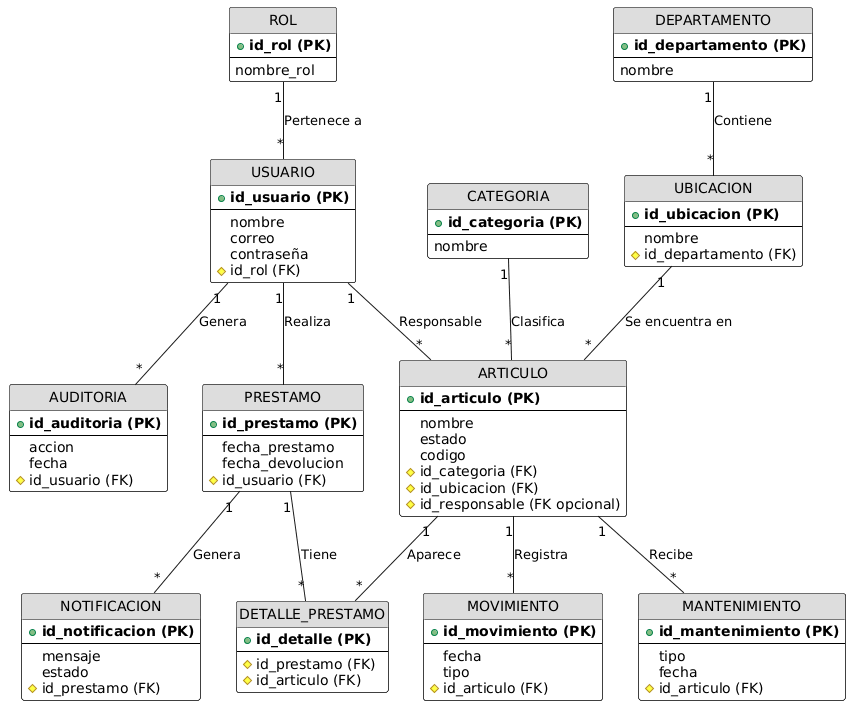
\includegraphics[width=0.9\textwidth]{imagenes/image1.png}
    \caption{Modelo Entidad-Relación}
    \label{fig:mer}
\end{figure}

\section{Modelo de Tablas con datos}

\begin{figure}[H]
    \begin{flushleft}
        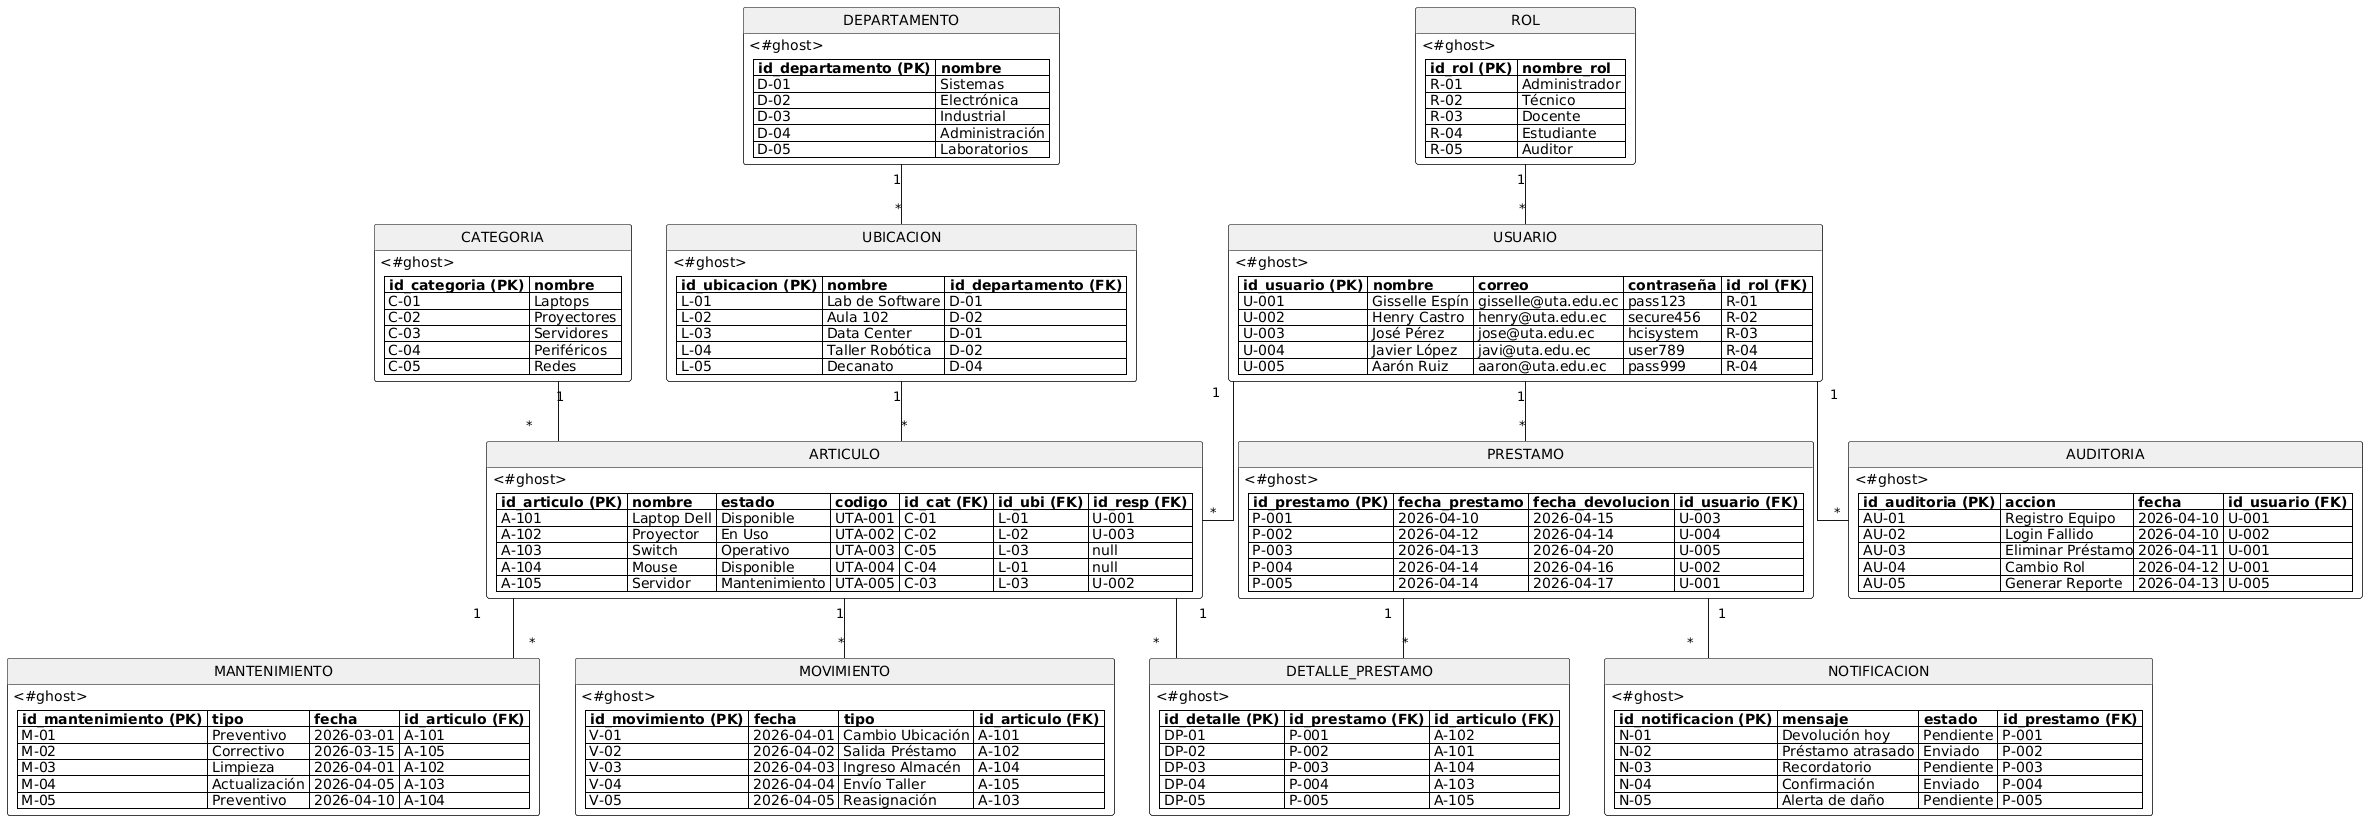
\includegraphics[width=18.5cm]{imagenes/image2.png} 
        
        \caption{Modelo relacional con datos de ejemplo}
        \label{fig:tablas}
    \end{flushleft}
\end{figure}
\section{Normalización del modelo}

El esquema propuesto se organiza hasta una estructura equivalente a la \textbf{Tercera Forma Normal (3FN)}, garantizando la eliminación de redundancias innecesarias y la integridad de los datos.

\subsection{Primera Forma Normal (1FN)}

En primer lugar, se asegura el cumplimiento de la \textbf{Primera Forma Normal (1FN)}, donde todas las tablas presentan atributos atómicos, es decir, cada campo almacena un solo valor y no existen grupos repetitivos. Por ejemplo, los artículos no almacenan múltiples categorías o ubicaciones en un mismo registro, sino que estas relaciones se gestionan mediante claves foráneas.

\subsection{Segunda Forma Normal (2FN)}

En la \textbf{Segunda Forma Normal (2FN)}, se eliminan dependencias parciales. Todas las tablas que poseen claves primarias compuestas, como \textbf{DETALLE\_PRESTAMO}, dependen completamente de su clave primaria. Esto evita que existan atributos que dependan solo de una parte de la clave, manteniendo coherencia en la estructura.

\subsection{Tercera Forma Normal (3FN)}

Finalmente, en la \textbf{Tercera Forma Normal (3FN)}, se eliminan dependencias transitivas. Ningún atributo no clave depende de otro atributo no clave. Por ejemplo, los datos de departamento no se almacenan en la tabla de artículos, sino en la entidad \textbf{DEPARTAMENTO}, relacionada mediante \textbf{UBICACION}, evitando duplicidad de información.

\subsection{Características adicionales}

\begin{itemize}
    \item Las entidades principales (\textbf{ARTICULO, USUARIO, PRESTAMO}) almacenan información de un solo contexto específico.
    \item Las entidades de catálogo (\textbf{ROL, CATEGORIA, DEPARTAMENTO}) permiten reutilización de datos y evitan redundancia.
    \item Las tablas transaccionales (\textbf{PRESTAMO, DETALLE\_PRESTAMO, MANTENIMIENTO, MOVIMIENTO, NOTIFICACION}) representan eventos del negocio.
    \item La integridad referencial se garantiza mediante el uso de claves foráneas correctamente definidas.
\end{itemize}

Esta organización mejora la \textbf{consistencia}, facilita el \textbf{mantenimiento del sistema} y permite una mayor \textbf{escalabilidad}, ya que la base de datos puede crecer sin generar inconsistencias ni duplicación de información.

\subsection{Habilidades blandas empleadas en la práctica}

\begin{itemize}
    \item[$\square$] Liderazgo
    \item[$\square$] Trabajo en equipo
    \item[$\square$] Comunicación asertiva
    \item[$\square$] La empatía
    \item[$\square$] Pensamiento crítico
    \item[$\square$] Flexibilidad
    \item[$\square$] La resolución de conflictos
    \item[$\square$] Adaptabilidad
    \item[$\square$] Responsabilidad
\end{itemize}
\subsection{Conclusiones}
El desarrollo del presente proyecto permitió estructurar de manera formal un sistema de gestión de inventario tecnológico, partiendo desde el levantamiento de requerimientos hasta la definición de un modelo relacional normalizado en 3FN, lo que garantiza consistencia y escalabilidad de los datos. La inclusión de entidades transaccionales como préstamos, mantenimientos y movimientos, junto con módulos de auditoría y notificaciones, demuestra que la solución propuesta es funcionalmente completa y adaptable a entornos reales de control de activos. La aplicación del modelo entidad-relación y su posterior transformación al modelo relacional permitió visualizar claramente las interacciones entre los distintos objetos del negocio, facilitando la detección de redundancias y la correcta asignación de claves primarias y foráneas. La validación mediante reglas de negocio y restricciones de integridad referencial asegura que el sistema mantendrá la calidad de la información incluso ante operaciones concurrentes o mal intencionadas. Finalmente, este trabajo sienta una base sólida para la implementación física en Oracle y el desarrollo de una interfaz web, cumpliendo así con los objetivos académicos y prácticos planteados al inicio de la asignatura.


\subsection{Recomendaciones}
Se recomienda que, antes de proceder con la implementación física en Oracle, los estudiantes realicen una validación conjunta del modelo relacional con un usuario experto del dominio, con el fin de ajustar detalles semánticos en los atributos y cardinalidades que podrían haber pasado desapercibidos en el análisis inicial. Es aconsejable definir de forma explícita los índices sobre las claves foráneas y los campos más consultados (como fechas de préstamo o estado de artículos) para optimizar el rendimiento de las consultas a medida que el volumen de datos crezca en producción. Para garantizar la seguridad del sistema, se debe implementar un control de acceso basado en roles (RBAC) desde la capa de base de datos, aprovechando las tablas USUARIO y ROL, y evitar la exposición de credenciales en el código fuente de la interfaz web. Se sugiere también automatizar, mediante triggers o procedimientos almacenados, la generación de registros de auditoría y el cambio de estado de los artículos al momento de registrar un préstamo o devolución, reduciendo así la carga lógica en la aplicación cliente. Por último, se recomienda documentar todas las restricciones CHECK, triggers y secuencias implementadas en Oracle, así como mantener un script de migración controlado que permita replicar fácilmente el esquema en entornos de prueba, desarrollo y producción.


\vspace{-3em} %reduce el espacio causado por refname vacío
\renewcommand{\refname}{}
\bibliographystyle{ieeetr}
\bibliography{sample}


\vfill

\end{document}